%!TEX root = arquiver6.tex

\newcommand*\circled[1]{\tikz[baseline=(char.base)]{
\node[shape=circle,draw,inner sep=0.7pt] (char) {#1};}}
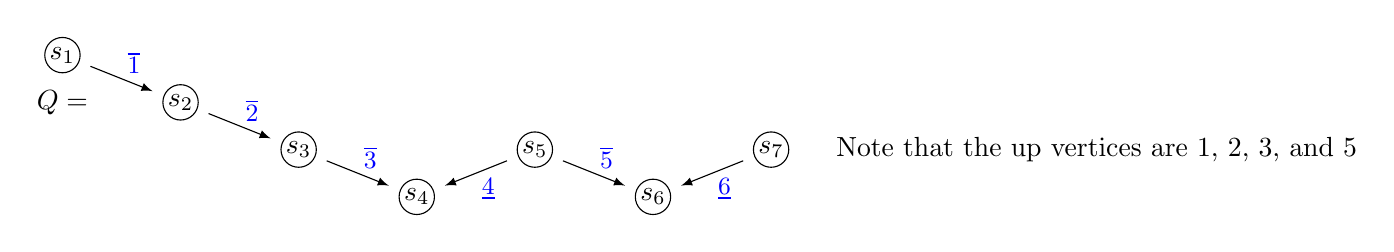
\begin{tikzpicture}[xscale=1.5,yscale=0.6,>=latex]%[scale=1.1,%line join=bevel,>=latex]
\draw (0,2) node {$Q=$};
\def\posetedgecolor{blue}
\node(1) at (0,3) {\circled{$s_{1}$}}; 
\node(2) at (1,2) {\circled{$s_{2}$}}; 
\node(3) at (2,1) {\circled{$s_{3}$}};  
\node(4) at (3,0) {\circled{$s_{4}$}};  
\node(5) at (4,1) {\circled{$s_{5}$}};   
\node(6) at (5,0) {\circled{$s_{6}$}}; 
\node(7) at (6,1) {\circled{$s_{7}$}}; 

\draw[->] (1) -- (2) node[\posetedgecolor,pos=0.7,above] {\small $\overline{1}$};

\draw[->]  (2) -- (3) node[\posetedgecolor,pos=0.7,above] {\small $\overline{2}$};

\draw[->] (3) -- (4) node[\posetedgecolor,pos=0.7,above] {\small $\overline{3}$}; 

\draw[<-] (4) -- (5) node[\posetedgecolor,pos=0.7,below] {\small $\underline{4}$}; 

\draw[->] (5) -- (6) node[\posetedgecolor,pos=0.7,above] {\small $\overline{5}$}; 

\draw[<-] (6) -- (7) node[\posetedgecolor,pos=0.7,below] {\small $\underline{6}$}; 

\draw (7) node[right=20pt] {Note that the up vertices are $1$, $2$, $3$, and $5$};

\end{tikzpicture}